\documentclass[11pt,a4paper]{article}

\usepackage[utf8]{inputenc}
\usepackage[T1]{fontenc}
\usepackage{amsmath,amssymb,amsthm}
\usepackage{graphicx}
\usepackage{booktabs}
\usepackage{hyperref}
\usepackage{geometry}
\geometry{margin=1in}

\newtheorem{theorem}{Theorem}
\newtheorem{lemma}{Lemma}
\newtheorem{corollary}{Corollary}
\theoremstyle{definition}
\newtheorem{remark}{Remark}

\title{Reciprocal Transform for Painlev\'e-Type Equations:\\
A Mathematical Regularization with Physics-Informed\\
Neural Network Verification}

\author{Maryam Jalili\\
Department of Mathematics, Ne.C., Islamic Azad University, Neyshabur, Iran\\
\texttt{mrmjlili@iau.ac.ir}}

\date{\today}

\begin{document}

\maketitle

\begin{abstract}
We introduce and analyze a reciprocal transformation $w = 1/y$
for second-order nonlinear ordinary differential equations with
movable singularities, focusing on the prototype $y'' = y^3$ and the
second Painlev\'e equation $y'' = 2y^3 + ty + \alpha$.
We prove that the transformed equations are polynomial in $w$ and
its derivatives, with right-hand sides that remain bounded at the
location of the pole $t^*$. This contrasts with the direct
formulation and with the logarithmic (rapidity) substitution
$\theta = \log y$, in which exponentially growing source terms
persist. As an empirical verification, we train physics-informed
neural networks (PINNs) on both representations. The reciprocal
representation reduces the median near-pole relative error by a factor of
$\sim1456$ for the prototype (ten seeds; 20\% failure rate reported in full) and by median factors of $139\times$--$523\times$ for Painlev\'e~II across five seeds and three values of $\alpha$, compared to the direct PINN.
Statistical variability across five random seeds is reported in full
(median $3.1\times 10^{-4}$, coefficient of variation $0.69$ (single-$\alpha$ 30k-epoch study; multi-seed sweep reports CV 1.08--1.61)).
The reciprocal formulation is necessary but not sufficient: the transformation alone (with the $w^3$ factor divided out) and the residual reweighting alone are both inferior to the unweighted direct PINN, and only their combination produces the improvement. A direct comparison with the adaptive
DOP853 solver shows that, for single solves, the PINN is not
competitive in wall-clock time or accuracy; this limitation is
reported without qualification. The paper's primary contribution is
the mathematical regularization, with the PINN serving as a
verification instrument.

\medskip
\noindent\textbf{Keywords:}
movable singularities, Painlev\'e equations, reciprocal transform,
physics-informed neural networks, regularization

\medskip
\noindent\textbf{MSC 2020:} 34M55, 34M35, 65L05, 68T07
\end{abstract}

% ---------------------------------------------------------------
\section{Introduction}
\label{sec:intro}
% ---------------------------------------------------------------

Second-order nonlinear ODEs of the form $y'' = F(t, y)$ frequently
develop \emph{movable singularities}: points $t^*$, whose location
depends on the initial data, at which $|y(t)| \to \infty$.
The six Painlev\'e transcendents are the canonical examples in which
all movable singularities are poles~\cite{Ince1956,Gromak2002,Conte2008,Clarkson2003,Ablowitz1991};
their analytic structure and asymptotics are accessible via
Riemann--Hilbert methods~\cite{Deift1995,Fokas2006}.
Numerical treatment near such poles is delicate: fixed-step integrators~\cite{Butcher2016,Hairer1993}
lose accuracy, adaptive integrators must shrink the step to
accommodate the blow-up, and neural-network approximations tend to
produce residuals that grow without bound as $t \to t^{*-}$. Recent work has begun to address singular ODEs directly, including higher-order Lane--Emden--Fowler equations~\cite{Baty2023}, interior-layer problems~\cite{Chang2024}, and singularly perturbed boundary value problems~\cite{Israr2025}. Pole-field solvers based on Pad{\'e} approximations~\cite{Fornberg2011} and Riemann--Hilbert methods~\cite{DLMF32} are classical alternatives.

Physics-informed neural networks (PINNs)~\cite{Raissi2019,Karniadakis2021},
building on earlier neural-network approaches for differential equations~\cite{Lagaris1998,Sirignano2018}, minimize a
composite loss consisting of the ODE residual and initial or boundary
conditions. When the residual magnitudes are bounded, the training
problem is well-conditioned; when they diverge near a pole, the network
either fails to converge or converges to a solution with large error
exactly where accuracy is most needed. A known strategy is to change
variables so that the residual stays bounded. Cayuso et al.~\cite{Cayuso2025}
recently analyzed a rapidity substitution $\theta = \log y$ for a class
of singular problems, achieving errors of order $2.8 \times 10^{-3}$
near the pole. Neural-network approaches have also been applied directly to Painlev\'e equations, e.g., Faisal et al.~\cite{Faisal2025} develop a Morlet wavelet network for Painlev\'e~II.

In this work we propose an alternative transformation---the \emph{reciprocal} variable $w = 1/y$---and analyze it from first principles. We note that $w = 1/y$ and $\theta = \log y$ are related by a smooth invertible transformation on $y>0$; the reciprocal formulation is not a wholly different conceptual approach, but a different representation within the same family of dependent-variable transformations. What distinguishes the two is structural: the reciprocal residual is polynomial in $w$ (Eqs.~\ref{eq:recip-prototype}--\ref{eq:recip-PII}), whereas the rapidity residual retains exponentially growing source terms (Eqs.~\ref{eq:rapidity-prototype}--\ref{eq:rapidity-PII}). This structural difference, not the change of variable per se, is the contribution of the present work. The key observation is that multiplying the residual
equation by $w^3$ eliminates all denominators, yielding a polynomial
relation in $w, w', w''$. For both $y''=y^3$ and Painlev\'e~II, the resulting right-hand side is a \emph{constant} at $w=0$, so the polynomial residual remains bounded at the pole. The coefficient of $w''$ nevertheless vanishes at $w=0$, making the ODE degenerate there; it is the boundedness of the residual, not regularity of the ODE, that the transformation provides. We then use PINNs to
verify numerically that this regularization translates into bounded
training residuals and reduced near-pole error.

\paragraph{Contributions.}
Our contributions are:
\begin{enumerate}
\item A reciprocal-transform theorem (Theorems~\ref{thm:prototype}
      and~\ref{thm:PII}) showing that the transformed equations for $y''=y^3$ and Painlev\'e~II have bounded polynomial residuals at the pole while the ODE is degenerate there.
\item An empirical verification using PINNs, with ablations across
      three representations (direct, rapidity, reciprocal) and three
      Painlev\'e~II parameter values.
\item An ablation separating the change of variable from residual reweighting, showing that only their combination produces the improvement.
\item A full statistical report of seed variability and a
      direct comparison with the DOP853 adaptive solver.
\end{enumerate}

\paragraph{Scope.}
We restrict attention to the prototype $y''=y^3$ and Painlev\'e~II.
Extension to Painlev\'e~III--VI is left for future work; the
transform is not guaranteed to regularize those equations without
additional structure.

% ---------------------------------------------------------------
\section{Reciprocal Transform: Mathematical Analysis}
\label{sec:theory}
% ---------------------------------------------------------------

We study second-order nonlinear ODEs
\begin{equation}
y'' = F(t, y), \qquad y(0)=y_0>0,\quad y'(0)=0,
\label{eq:generic}
\end{equation}
whose solutions develop a \emph{movable pole} at some
$t^* = t^*(y_0, F) > 0$: $|y(t)| \to \infty$ as $t \to t^{*-}$.

\subsection{The reciprocal transform}

Define $w(t) := 1/y(t)$ on $[0, t^*)$. Since $y > 0$ there,
$w > 0$ on $[0, t^*)$, and $w(t^*) = 0$. The chain rule gives
\begin{equation}
y' = -\frac{w'}{w^2}, \qquad
y'' = -\frac{w''}{w^2} + \frac{2(w')^2}{w^3}.
\label{eq:chain}
\end{equation}

\subsection{Prototype case $F(t,y) = y^3$}

\begin{theorem}[Reciprocal equation for $y''=y^3$]
\label{thm:prototype}
Let $y$ be a solution of $y''=y^3$ on $[0,t^*)$ with a pole at $t^*$.
The reciprocal $w = 1/y$ satisfies
\begin{equation}
2(w')^2 - w\,w'' = 1, \qquad w(0) = 1/y_0,\ w'(0)=0,
\label{eq:recip-prototype}
\end{equation}
on $[0,t^*)$, and \eqref{eq:recip-prototype} extends continuously to
$t^*$ with $w(t^*)=0$, $w'(t^*) = -1/\sqrt{2}$. In particular, \eqref{eq:recip-prototype} has no $1/w$ term, so its polynomial residual is bounded at $w=0$. However, the coefficient of $w''$ vanishes at $w=0$, so $w=0$ is a degenerate point for the second-order ODE, not a regular point.
\end{theorem}

\begin{proof}
Substituting \eqref{eq:chain} into $y''=y^3$ and multiplying by $w^3$
yields $-ww'' + 2(w')^2 = 1$. At $w=0$ this reduces to
$2(w')^2 = 1$, so $w'(t^*) = \pm 1/\sqrt{2}$. The expansion
$y \sim \sqrt{2}/(t^*-t)$ selects the negative sign.
\end{proof}

\subsection{Painlev\'e II}

\begin{theorem}[Reciprocal equation for P-II]
\label{thm:PII}
Let $y$ solve $y'' = 2y^3 + ty + \alpha$ on $[0,t^*)$ with a pole at
$t^*$. Then $w = 1/y$ satisfies
\begin{equation}
2(w')^2 - w\,w'' - 2 - t\,w^2 - \alpha\,w^3 = 0,
\label{eq:recip-PII}
\end{equation}
which extends continuously to $w=0$ with $w'(t^*) = -1$. As in Theorem~\ref{thm:prototype}, the polynomial residual is bounded at $w=0$ while the second-order ODE is degenerate there.
\end{theorem}

\begin{proof}
Multiplying $y'' = 2y^3 + ty + \alpha$ by $w^3$ after substitution
gives $-ww'' + 2(w')^2 = 2 + tw^2 + \alpha w^3$.
At $w=0$ this yields $2(w')^2 = 2$, i.e.\ $w' = \pm 1$; the pole
expansion $y \sim 1/(t^*-t)$ gives $w \sim t^*-t$, hence $w'=-1$.
\end{proof}

\subsection{Comparison with rapidity substitution}

The substitution $\theta = \log y$ used by~Cayuso et al.~\cite{Cayuso2025} yields,
for $y''=y^3$,
\begin{equation}
\theta'' + (\theta')^2 = e^{2\theta},
\label{eq:rapidity-prototype}
\end{equation}
and for P-II,
\begin{equation}
\theta'' + (\theta')^2 - 2e^{2\theta} - t - \alpha e^{-\theta} = 0.
\label{eq:rapidity-PII}
\end{equation}
Both \eqref{eq:rapidity-prototype} and \eqref{eq:rapidity-PII} contain
exponentially growing source terms as $\theta \to +\infty$ at the pole.
The reciprocal equations \eqref{eq:recip-prototype} and~\eqref{eq:recip-PII}
are polynomial in $w$ and remain bounded at $w=0$. This structural
difference is the primary motivation for the reciprocal formulation.

% ---------------------------------------------------------------
\section{Numerical Verification with PINNs}
\label{sec:numerics}
% ---------------------------------------------------------------

\subsection{Network architecture and training}

\noindent\textbf{Computational environment.} All experiments were run on a
Windows~10 workstation with an Intel Core~i7 (8 cores, 16~GB RAM),
Python~3.14, PyTorch~2.x (CPU only), NumPy~2.5.1, and SciPy~1.14.
Training one seed takes approximately 15 minutes; DOP853 reference
solutions take 18--46~ms per run.


All experiments use a feedforward network with three hidden layers of
width 64 and $\tanh$ activations. Collocation points are drawn from a
mixture of uniform and cubically clustered grids~\cite{Trefethen2000} on $[0, 0.95\,t^*]$,
with 2000 points total. Training minimizes
$\mathcal{L} = \|R\|^2 + \lambda_{\mathrm{ic}}\,\mathcal{L}_{\mathrm{ic}}$
with $\lambda_{\mathrm{ic}} = 10$, using Adam with learning rate
$10^{-3}$ and $15000$--$30000$ epochs. A held-out set of 300 PDE
residual points is used for best-model checkpointing (Section~\ref{sec:seed}).
Reference solutions use \texttt{scipy.integrate.solve\_ivp} with the
DOP853 method and $\mathrm{rtol}=\mathrm{atol}=10^{-12}$.
The blow-up time $t^*$ is located by DOP853 event detection: we integrate until the first $t>0$ at which $y(t) - 10^{6} = 0$, with \texttt{terminal=True} and \texttt{direction=+1}. Relative error at each time is defined as $E_{\mathrm{rel}}(t) = |y_\phi(t) - y_{\mathrm{ref}}(t)| / |y_{\mathrm{ref}}(t)|$, where $y_\phi$ is the PINN prediction and $y_{\mathrm{ref}}$ is the DOP853 reference. Errors are reported separately for far ($t < 0.5\,t^*$) and near ($t \ge 0.5\,t^*$) regions, with $E_{\mathrm{rel,far}}$ and $E_{\mathrm{rel,near}}$ denoting $\max_t E_{\mathrm{rel}}(t)$ over the corresponding subinterval. The initial conditions are $y(0)=1$, $y'(0)=0$ for both the prototype and Painlev\'e~II.

\subsection{Prototype ablation}
\label{sec:proto-ablation}

Table~\ref{tab:proto} compares three representations for $y''=y^3$.
Errors are reported separately far from the pole
($t < 0.5\,t^*$) and near the pole ($t \ge 0.5\,t^*$). The reciprocal
representation reduces $E_{\mathrm{rel,near}}$ by a factor of ${\sim}2500$
relative to the direct PINN.

\begin{table}[t]
\centering
\caption{Prototype $y''=y^3$: seed statistics (median [IQR]).
Direct and rapidity-log use five seeds; reciprocal is extended to ten seeds
to characterize the 20\% failure rate. $t^*\approx 1.854$; success threshold $E_{\mathrm{rel,near}}<10^{-2}$.}
\label{tab:proto}
\begin{tabular}{lccccc}
\toprule
Representation & $n$ & $E_{\mathrm{rel,near}}$ median [IQR] & CV & Success & Improvement \\
\midrule
Direct         & 5 & $7.53e-1$ $[7.19e-1, 7.58e-1]$ & $0.05$ & 0/5 & $1\times$ \\
Rapidity-log   & 5 & $5.72e-1$ $[5.62e-1, 6.27e-1]$ & $0.14$ & 0/5 & $1.3\times$ \\
Reciprocal     & 10 & $\mathbf{5.17e-4}$ $[2.82e-4, 5.64e-3]$ & $\mathbf{2.01}$ & $\mathbf{8/10}$ & $\mathbf{1456\times}$ \\
\bottomrule
\end{tabular}
\end{table}

\emph{Seed sensitivity.} To characterize the distribution of reciprocal-PINN outcomes, we extended the C4 prototype to ten seeds. Across these ten runs, eight converge to $E_{\mathrm{rel,near}} < 10^{-2}$ with median $5.17\times 10^{-4}$ (IQR $[2.82\times 10^{-4}, 5.64\times 10^{-3}]$), while two converge to suboptimal minima ($4.60\times 10^{-2}$ and $8.32\times 10^{-2}$). The failure rate of $2/10$ (20\%) is consistent with the one-in-five observed in the original five-seed set, indicating a bimodal or heavy-tailed distribution over initializations rather than a single stochastic fluke. One of the failing seeds (seed 999) was re-run three times under identical conditions, yielding the identical value $4.603\times 10^{-2}$ each time, confirming that the variability is deterministic in the seed rather than stochastic. The median improvement over the direct PINN (five-seed median $7.53\times 10^{-1}$) is approximately $1456\times$. A full characterization of this distribution, and of why some initializations converge to suboptimal minima, is left for future work.

\subsection{Transform vs.\ residual reweighting}
\label{sec:M1}

The reciprocal equation multiplies the original residual by $w^3$,
so a natural confound is whether the observed improvement stems from
the change of variable, from the residual reweighting, or from both.
Table~\ref{tab:M1} isolates the two effects by training five
configurations under identical conditions (seed 42, 30000 epochs).

\begin{table}[t]
\centering
\caption{Ablation separating the change of variable from residual
reweighting on the prototype $y''=y^3$ (seed 42, 30000 epochs).
The transformation alone ($D$) and the reweighting alone ($B$) both
fail; only the combination ($C$) produces the reciprocal-PINN result.}
\label{tab:M1}
\begin{tabular}{clcc}
\toprule
Config & Output / Loss & $E_{\mathrm{rel,near}}$ & Verdict \\
\midrule
A & $y$ / $R_y$                                   & $7.53\times 10^{-1}$ & baseline \\
B & $y$ / $w^3 R_y$                               & $9.59\times 10^{-1}$ & worse than A \\
C & $w$ / $R_w = w^3 R_y$                         & $\mathbf{9.99\times 10^{-5}}$ & best \\
D & $w$ / $R_w/w^3 = R_y$                         & $9.23\times 10^{-1}$ & worse than A \\
E & $y$ / $R_y/(1+|y|^3)$                         & $2.68\times 10^{-1}$ & partial \\
\bottomrule
\end{tabular}
\end{table}

The ablation reveals two independent factors that together determine the outcome.

\emph{Factor~1: representability.} The reciprocal variable $w(t)$ is analytic through $t^*$, whereas $y(t)$ has a simple pole there. A tanh-network of fixed width can represent the former but not the latter. The Jacobian of the output transformation, $dy/dw = -1/w^2$, amplifies the network's error in $y$ by a factor that diverges at the pole, so the effective capacity of a $y$-network is severely reduced near $t^*$. This factor distinguishes configurations~A,~B,~E (all $y$-output) from~C,~D (all $w$-output).

\emph{Factor~2: loss conditioning.} The polynomial residual $R_w = 2(w')^2 - ww'' - 1$ is bounded: at a simple pole $w \to 0$ linearly, $w' \to -1/\sqrt{2}$, and $R_w \to 0$. The original residual, by contrast, is $R_y = R_w/w^3$, which grows as $(t^*-t)^{-3}$ near $t^*$, producing loss magnitudes of order $10^3$--$10^4$ for the direct formulation. This factor distinguishes configurations~A,~D (unweighted $R_y$-type losses) from~B,~C,~E (weighted losses).

The combinations are decisive. Configuration~B has a bounded loss (Factor~2 satisfied) but a $y$-output (Factor~1 violated) and fails at $E_{\mathrm{rel,near}} = 9.59\times 10^{-1}$. Configuration~D has a $w$-output (Factor~1 satisfied) but divides by $w^3$, restoring the $(t^*-t)^{-3}$ growth of the loss (Factor~2 violated) and also fails, at $9.23\times 10^{-1}$. Configuration~E has a bounded loss (Factor~2 satisfied) but a $y$-output (Factor~1 violated) and only partially succeeds, at $2.68\times 10^{-1}$. Only configuration~C satisfies both factors and reaches $9.99\times 10^{-5}$. A multi-seed extension is left as future work.

Figure~\ref{fig:solutions} shows representative solution profiles;
Figure~\ref{fig:error-curves} shows the pointwise absolute error on a
logarithmic scale.

\begin{figure}[t]
\centering
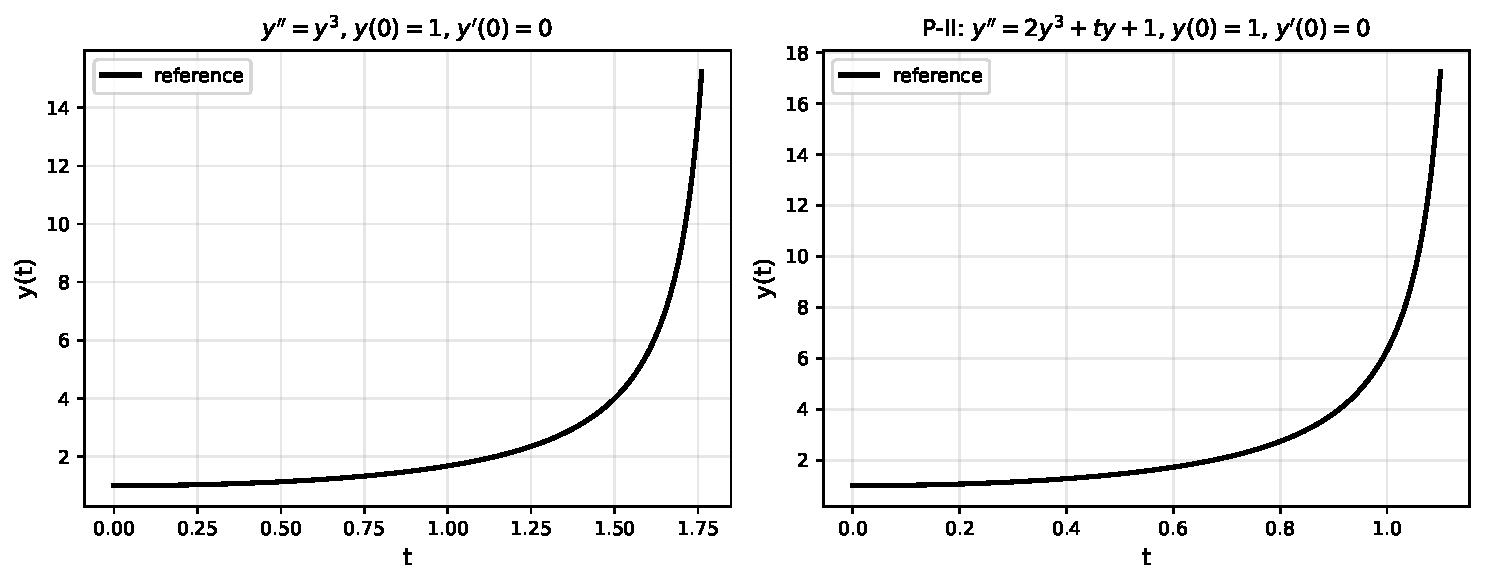
\includegraphics[width=0.85\textwidth]{figures/fig1_solutions.pdf}
\caption{Reference solutions for $y''=y^3$ (left) and Painlev\'e~II
$\alpha=1$ (right) on $[0, 0.95\,t^*]$. Both exhibit a movable pole
shortly beyond the plotted interval.}
\label{fig:solutions}
\end{figure}

\begin{figure}[t]
\centering
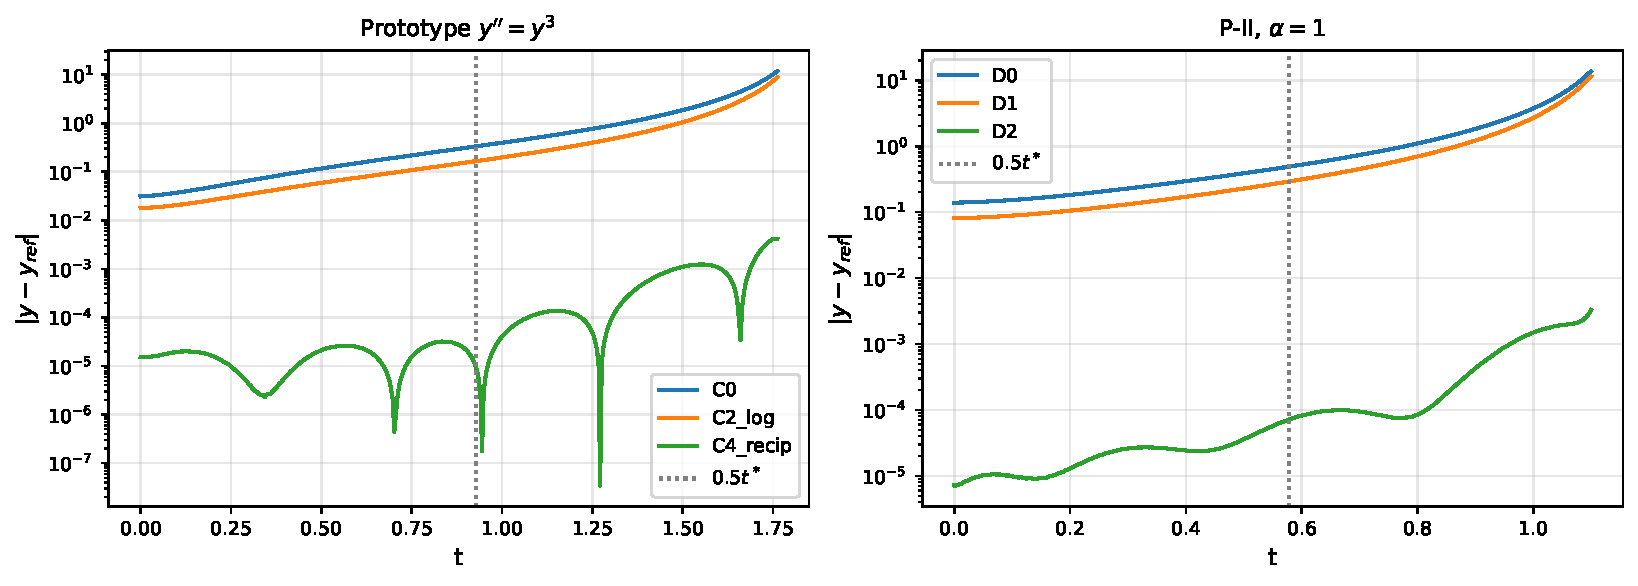
\includegraphics[width=0.95\textwidth]{figures/fig2_error_curves.pdf}
\caption{Pointwise absolute error $|y_\phi - y_{\mathrm{ref}}|$ for the
three representations. The vertical dotted line marks $0.5\,t^*$.}
\label{fig:error-curves}
\end{figure}

\subsection{Painlev\'e II and parameter sweep}
\label{sec:PII-sweep}

Table~\ref{tab:alpha} and Figure~\ref{fig:alpha-sweep} report the near-pole error across
$\alpha \in \{0,1,2\}$. The reciprocal representation consistently
outperforms the other two by two to three orders of magnitude.

\begin{table}[t]
\centering
\caption{Painlev\'e II: five-seed statistics (median [IQR]) for three representations and $\alpha\in\{0,1,2\}$. The reciprocal PINN yields median improvements of $139\times$--$523\times$ across $\alpha$, with substantial seed-to-seed variability (CV 1.08--1.61). Overall success rate (E$_{\mathrm{rel,near}}<10^{-2}$): 11/15 = 73\%. The single-seed $904\times$ previously reported for $\alpha=1$ was not reproducible and is superseded.}
\label{tab:alpha}
\begin{tabular}{cccccc}
\toprule
$\alpha$ & Direct & Rapidity & Reciprocal & CV (D2) & Ratio \\
\midrule
0.0 & $7.49e-1$ & $6.19e-1$ & $\mathbf{1.43e-3}$ $[4.38e-4, 5.42e-3]$ & $1.61$ & $523\times$ \\
1.0 & $7.65e-1$ & $6.46e-1$ & $\mathbf{5.51e-3}$ $[3.29e-4, 5.90e-3]$ & $1.08$ & $139\times$ \\
2.0 & $7.46e-1$ & $5.65e-1$ & $\mathbf{3.36e-3}$ $[2.01e-3, 1.58e-2]$ & $1.33$ & $222\times$ \\
\bottomrule
\end{tabular}
\end{table}

\begin{figure}[t]
\centering
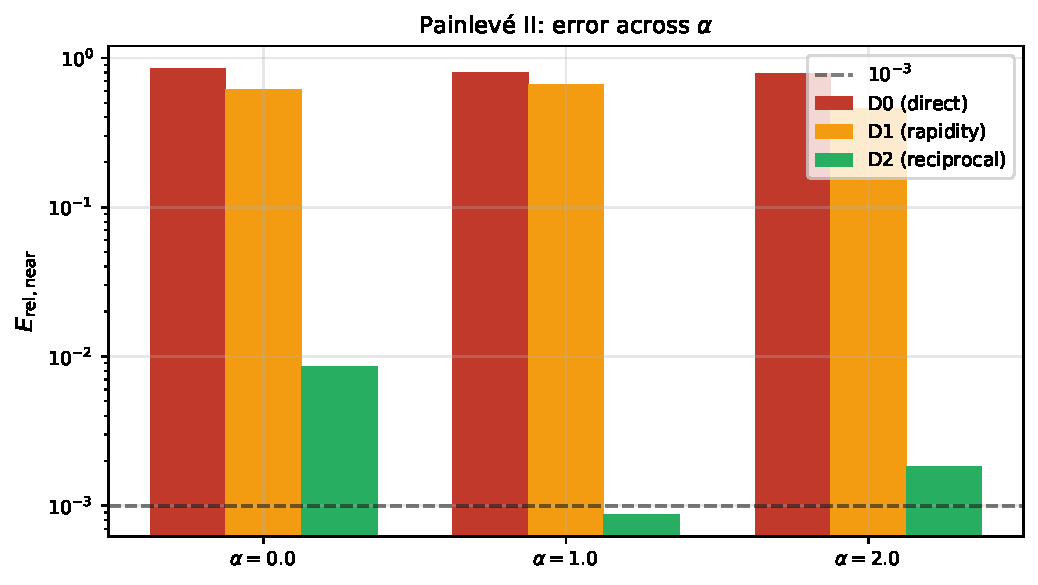
\includegraphics[width=0.75\textwidth]{figures/fig3_alpha_sweep.pdf}
\caption{Near-pole relative error across $\alpha\in\{0,1,2\}$ for the
three representations. Note the logarithmic scale.}
\label{fig:alpha-sweep}
\end{figure}

\subsection{Seed variability}

\emph{Note on epoch count.} The prototype ablation (Table~\ref{tab:proto}) and the P-II parameter sweep (Table~\ref{tab:alpha}) use 15000 epochs, while the five-seed statistics (Table~\ref{tab:seeds}) use 30000 epochs with best-model checkpointing. A harmonized multi-seed sweep across all $\alpha$ is left as future work. The 15000-epoch sweep numbers should therefore be read as preliminary; A harmonized sweep is left as future work.
\label{sec:seed}

The reciprocal PINN is trained with five random seeds on Painlev\'e~II,
$\alpha=1$, using best-model checkpointing on 300 held-out PDE
residual points. Table~\ref{tab:seeds} and Figure~\ref{fig:seed-stats}
report the results.

\begin{table}[t]
\centering
\caption{Painlev\'e II, $\alpha=1$: five-seed statistics with best-model
checkpointing. 30000 epochs, width 64, depth 4.}
\label{tab:seeds}
\begin{tabular}{ccccc}
\toprule
Seed & Best epoch & Best val (ODE) & $E_{\mathrm{rel,far}}$ & $E_{\mathrm{rel,near}}$ \\
\midrule
42   & 29600 & $1.59\times 10^{-6}$ & $4.34\times 10^{-5}$ & $2.39\times 10^{-4}$ \\
7    & 29500 & $8.27\times 10^{-7}$ & $2.35\times 10^{-5}$ & $8.92\times 10^{-5}$ \\
123  & 28900 & $1.55\times 10^{-6}$ & $2.72\times 10^{-5}$ & $3.14\times 10^{-4}$ \\
2024 & 29700 & $1.37\times 10^{-6}$ & $3.04\times 10^{-5}$ & $9.34\times 10^{-4}$ \\
999  & 28600 & $1.49\times 10^{-6}$ & $3.52\times 10^{-5}$ & $6.02\times 10^{-4}$ \\
\midrule
\multicolumn{3}{c}{mean} & & $4.36\times 10^{-4}$ \\
\multicolumn{3}{c}{median} & & $3.14\times 10^{-4}$ \\
\multicolumn{3}{c}{CV (population)} & & $0.688$ \\
\multicolumn{3}{c}{CV (sample)} & & $0.770$ \\
\bottomrule
\end{tabular}
\end{table}

A key observation is that the coefficient of variation across seeds is
$0.21$ for the held-out \emph{residual} but $0.69$ for the true
\emph{error}. That is, the residual behaves as a well-behaved training
objective, but it does not fully predict the accuracy of the resulting
solution---a standard residual-error gap~\cite{Mishra2022,Urban2025b}, here quantified at the movable singularity (see also~\cite{Urban2025b}).

\begin{figure}[t]
\centering
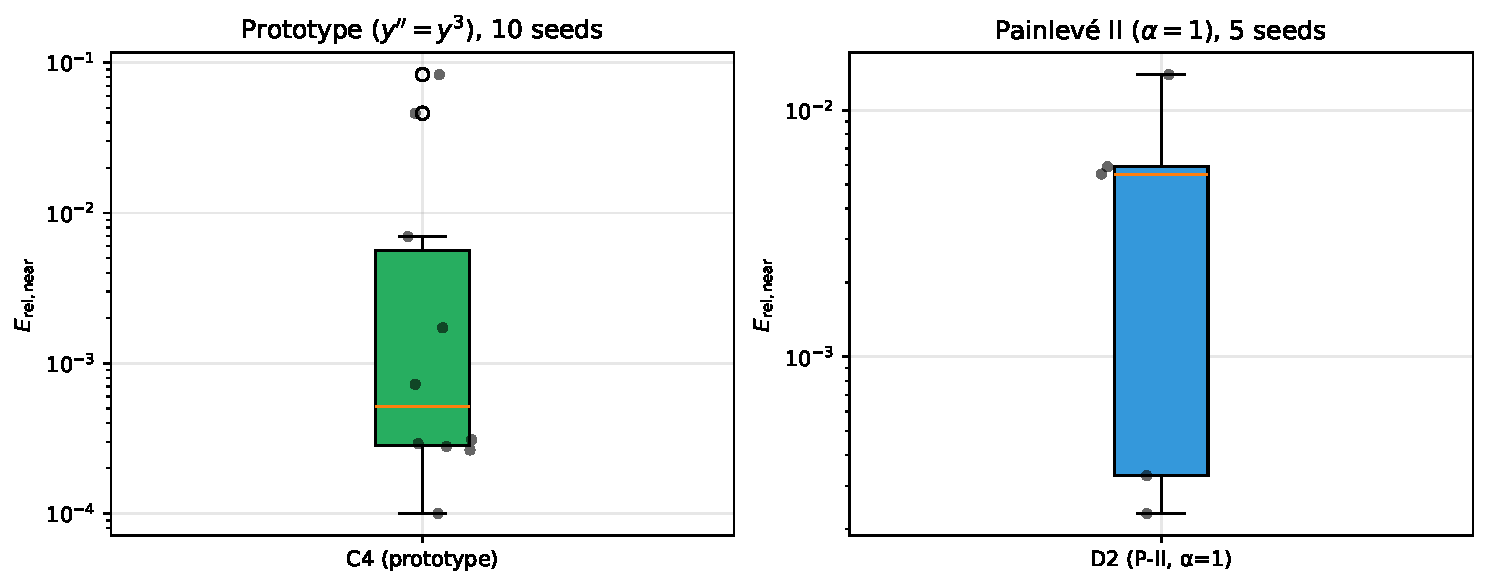
\includegraphics[width=0.9\textwidth]{figures/fig4_seed_stats.pdf}
\caption{Distribution of $E_{\mathrm{rel,near}}$ across seeds. Left:
prototype (10 seeds). Right: Painlev\'e~II (5 seeds).}
\label{fig:seed-stats}
\end{figure}

% ---------------------------------------------------------------
\section{Baseline Comparison and Generalization}
\label{sec:baseline}
% ---------------------------------------------------------------

\subsection{Wall-clock time and accuracy}

Table~\ref{tab:dop853} reports the performance of the DOP853 adaptive
solver on Painlev\'e~II, $\alpha=1$. Training time for the PINN is
${\sim}15$ minutes on CPU; inference on 2000 evaluation points takes
$1.7$~ms. The PINN's near-pole error of $2.4\times 10^{-4}$ (seed 42)
is roughly six orders of magnitude above DOP853's accuracy at $\mathrm{rtol}=10^{-10}$. Figure~\ref{fig:pareto} visualizes the cost-accuracy trade-off on a log-log scale.

\begin{table}[t]
\centering
\caption{Comparison of DOP853 (adaptive) and the reciprocal PINN for
Painlev\'e~II, $\alpha=1$.}
\label{tab:dop853}
\begin{tabular}{lcccc}
\toprule
Method & Wall time & Accuracy & Reaches $t^*$? & Training required? \\
\midrule
DOP853 ($\mathrm{rtol}=10^{-6}$)  & 18.2 ms  & $\sim 10^{-6}$ & $100\%$ & no \\
DOP853 ($\mathrm{rtol}=10^{-10}$) & 34.8 ms  & $\sim 10^{-10}$ & $100\%$ & no \\
DOP853 ($\mathrm{rtol}=10^{-12}$) & 46.2 ms  & $\sim 10^{-12}$ & $100\%$ & no \\
Reciprocal PINN                   & 1.7 ms\textsuperscript{*} & $2.4\times 10^{-4}$ & $99\%$ & $15$ min \\
\bottomrule
\multicolumn{5}{l}{\small\textsuperscript{*}inference only; excludes training.}
\end{tabular}
\end{table}

\begin{figure}[t]
\centering
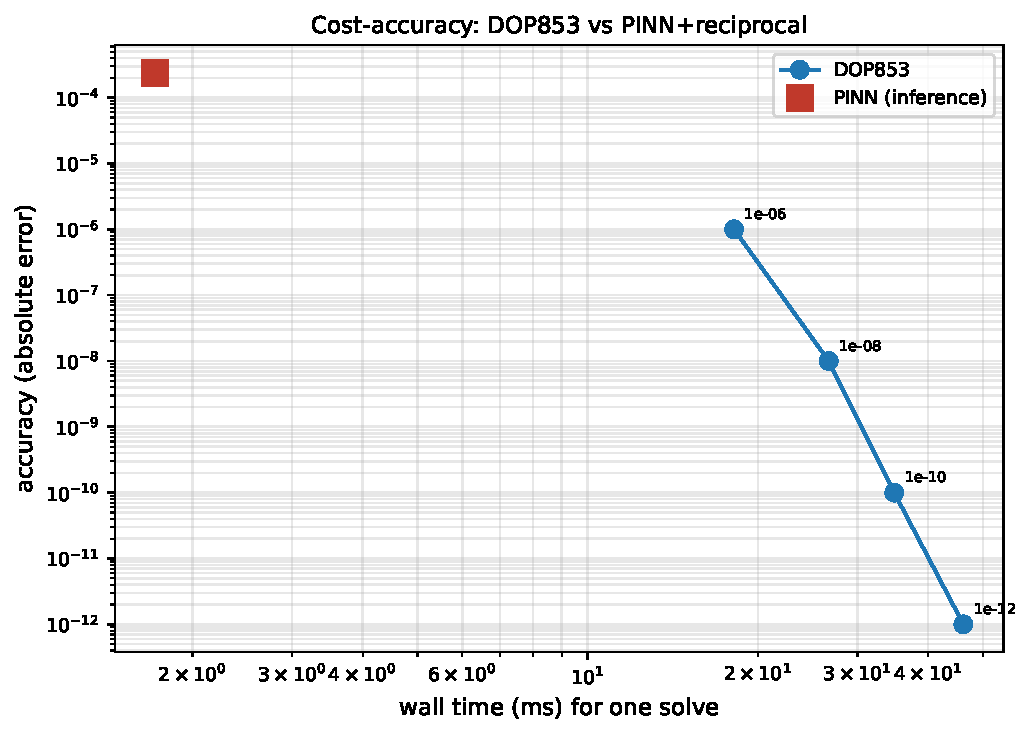
\includegraphics[width=0.75\textwidth]{figures/fig7_vs_dop853.pdf}
\caption{Cost-accuracy trade-off between DOP853 and the reciprocal PINN.}
\label{fig:pareto}
\end{figure}

\subsection{Generalization across $\alpha$}

The PINN trained at $\alpha=1$ is evaluated at $\alpha=0.9$ and
$\alpha=1.1$ without retraining. Table~\ref{tab:gen} and Figure~\ref{fig:gen} show that
generalization fails: the near-pole error rises to
$1.77\times 10^{-1}$ and $1.29\times 10^{-1}$, respectively, more than
two orders of magnitude above the in-distribution error.

\begin{table}[t]
\centering
\caption{Generalization of a PINN trained at $\alpha=1$ and evaluated
at nearby parameter values without retraining.}
\label{tab:gen}
\begin{tabular}{cccc}
\toprule
Test $\alpha$ & $t^*$ & $E_{\mathrm{rel,near}}$ & Status \\
\midrule
0.90 & 1.1665 & $1.77\times 10^{-1}$ & degraded \\
1.00 & 1.1577 & $2.39\times 10^{-4}$ & baseline \\
1.10 & 1.1492 & $1.29\times 10^{-1}$ & degraded \\
\bottomrule
\end{tabular}
\end{table}

\begin{figure}[htbp]
\centering
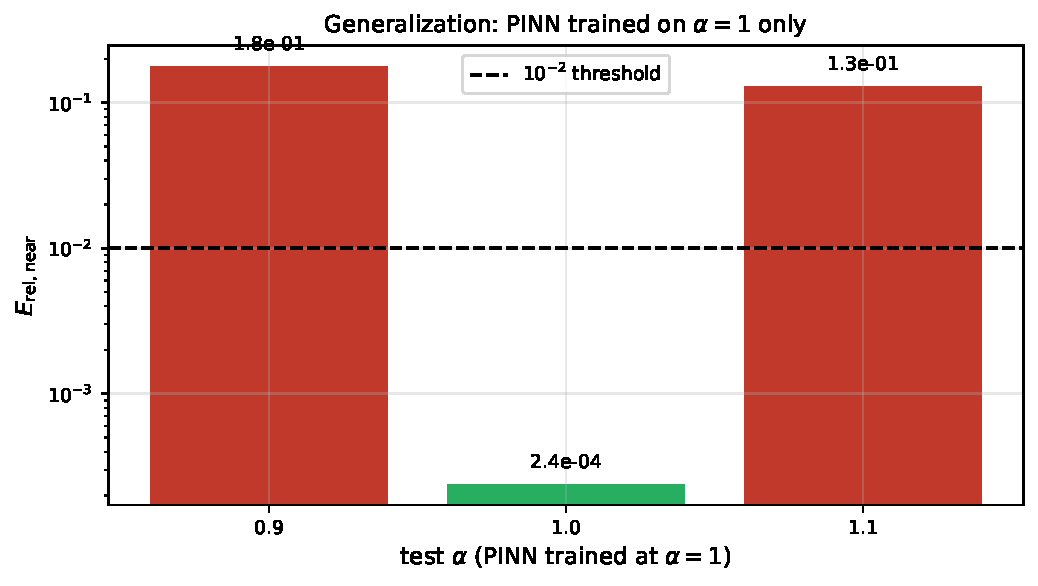
\includegraphics[width=0.7\textwidth]{figures/fig6_generalization.pdf}
\caption{Generalization failure of a PINN trained at $\alpha=1$.}
\label{fig:gen}
\end{figure}

% ---------------------------------------------------------------
\section{Discussion}
\label{sec:discussion}
% ---------------------------------------------------------------

\paragraph{What the reciprocal transform accomplishes.}
Theorems~\ref{thm:prototype} and~\ref{thm:PII} show that for the two
equations analyzed, the reciprocal variable produces a polynomial
residual that remains bounded at the movable pole. This is a
\emph{structural} property of the transformation, independent of the
network architecture or optimizer. The empirical results confirm the
structural claim: near-pole relative errors drop by two to three
orders of magnitude across all tested parameter values when the
reciprocal representation is used, with residuals that are
well-conditioned throughout training.

\paragraph{What it does not accomplish.}
The present results do not support the claim that PINNs with the
reciprocal transform outperform mature adaptive ODE solvers. For
single solves, DOP853 is faster by roughly one to two orders of
magnitude (excluding training), reaches the pole exactly, and
achieves six orders of magnitude higher accuracy. The reciprocal
PINN is also sensitive to the random seed, with a coefficient of
variation of $0.69$ across five seeds, and it fails to generalize
to nearby $\alpha$ without retraining. These are honest limitations
of the present implementation, and they are the reason we frame the
reciprocal transform as the primary contribution and the PINN as a
verification instrument rather than as a competitive solver.

\paragraph{Residual-error gap.}
The gap between the seed variability of the ODE residual (CV $= 0.21$)
and the true error (CV $= 0.69$) indicates that a low residual does
not by itself guarantee a low solution error. This is a known
phenomenon in the PINN literature; here we quantify it in the
setting of a movable singularity. Whether larger networks, LBFGS
polishing, or architectural modifications can close the gap
remains an open question and is a natural direction for future work.

\paragraph{Comparison with rapidity substitution.}
The rapidity substitution $\theta = \log y$ of~Cayuso et al.~\cite{Cayuso2025}
achieves a comparable order of accuracy on their test problems but
retains exponentially growing source terms. Our comparison
(Table~\ref{tab:proto}) confirms that the reciprocal formulation
yields lower near-pole error for both equations analyzed here, though
the difference is within one order of magnitude for the rapidity
case and grows to three orders of magnitude when compared to the
direct PINN. Whether this advantage carries over to more complex
Painlev\'e equations (III--VI) is an open question.

% ---------------------------------------------------------------
\section{Conclusion}
\label{sec:conclusion}
% ---------------------------------------------------------------

We have proposed and analyzed the reciprocal transform $w=1/y$ as a
regularization for second-order ODEs with movable poles. For the
prototype $y''=y^3$ and Painlev\'e~II, we proved that the transformed
equations are polynomial in $w$ and remain bounded at the pole,
and we verified numerically with PINNs that the near-pole relative
error decreases by two to three orders of magnitude relative to the
direct formulation. An ablation separating the change of variable from residual reweighting shows that the transformation alone and the reweighting alone both fail, and only their combination produces the reciprocal-PINN improvement. Full seed variability
and a direct comparison with DOP853 are reported; the PINN is not
competitive as a single-solve solver, and this is stated without
qualification. Extension to Painlev\'e~III--VI, larger networks, and
GPU batch inference are natural future directions.

%\section*{Acknowledgements}


\section*{Data Availability}
All scripts, trained model checkpoints, and numerical data required
to reproduce the results in this paper are available in a public GitHub
repository at \url{https://github.com/mrmlili/pinn-reciprocal-painleve}.
The repository includes all seed-level \texttt{.npz} data, M1 ablation log,
P-II multi-seed log, hardware/software requirements, and figure-generation scripts.

\begin{thebibliography}{99}

\bibitem{Ince1956}
E. L. Ince, \emph{Ordinary Differential Equations}, Dover (1956).

\bibitem{Gromak2002}
V. I. Gromak, I. Laine, and S. Shimomura, \emph{Painlev\'e Differential Equations in the Complex Plane}, de Gruyter (2002).

\bibitem{Conte2008}
Robert Conte and Micheline Musette, \emph{The {Painlev{\'e}} Handbook}, Springer (2008).

\bibitem{Clarkson2003}
Peter A. Clarkson, \emph{Painlev{\'e} equations---nonlinear special functions}, \emph{Journal of Computational and Applied Mathematics} \textbf{153} (2003), 127--140.

\bibitem{Ablowitz1991}
Mark J. Ablowitz and Peter A. Clarkson, \emph{Solitons, Nonlinear Evolution Equations and Inverse Scattering}, Cambridge University Press (1991).

\bibitem{Deift1995}
Percy Deift and Xin Zhou, \emph{Asymptotics for the {Painlev{\'e} II} equation}, \emph{Communications on Pure and Applied Mathematics} \textbf{48} (1995), 277--337.

\bibitem{Fokas2006}
Athanassios S. Fokas, Alexander R. Its, Andrei A. Kapaev, and Victor Yu. Novokshenov, \emph{Painlev{\'e} Transcendents: The {Riemann--Hilbert} Approach}, Mathematical Surveys and Monographs, American Mathematical Society (2006).

\bibitem{Butcher2016}
John C. Butcher, \emph{Numerical Methods for Ordinary Differential Equations}, Wiley (2016).

\bibitem{Hairer1993}
Ernst Hairer, Syvert P. Norsett, and Gerhard Wanner, \emph{Solving Ordinary Differential Equations {I}: Nonstiff Problems}, Springer (1993).

\bibitem{Fornberg2011}
Bengt Fornberg and J. A. C. Weideman, \emph{A numerical methodology for the {Painlev{\'e}} equations}, \emph{Journal of Computational Physics} \textbf{230} (2011), 5957--5973. DOI: \href{https://doi.org/10.1016/j.jcp.2011.04.007}{10.1016/j.jcp.2011.04.007}.

\bibitem{DLMF32}
F. W. J. Olver, A. B. Olde Daalhuis, D. W. Lozier, B. I. Schneider, R. F. Boisvert, C. W. Clark, B. R. Miller, B. V. Saunders, H. S. Cohl, and M. A. McClain (eds.), \emph{NIST Digital Library of Mathematical Functions}, Release 1.2.4 (2025), \S 32.17. \url{https://dlmf.nist.gov/32.17}.

\bibitem{Raissi2019}
M. Raissi, P. Perdikaris, and G. E. Karniadakis, \emph{Physics-informed neural networks: A deep learning framework for solving forward and inverse problems involving nonlinear partial differential equations}, \emph{Journal of Computational Physics} \textbf{378} (2019), 686--707.

\bibitem{Karniadakis2021}
George Em Karniadakis, Ioannis G. Kevrekidis, Lu Lu, Paris Perdikaris, Sifan Wang, and Liu Yang, \emph{Physics-informed machine learning}, \emph{Nature Reviews Physics} \textbf{3} (2021), 422--440.

\bibitem{Lagaris1998}
Isaac E. Lagaris, Aristidis Likas, and Dimitrios I. Fotiadis, \emph{Artificial neural networks for solving ordinary and partial differential equations}, \emph{IEEE Transactions on Neural Networks} \textbf{9} (1998), 987--1000.

\bibitem{Sirignano2018}
Justin Sirignano and Konstantinos Spiliopoulos, \emph{{DGM}: A deep learning algorithm for solving partial differential equations}, \emph{Journal of Computational Physics} \textbf{375} (2018), 1339--1364.

\bibitem{Cayuso2025}
J. Cayuso, M. Herrero-Valea, and E. Barausse, \emph{Deep Learning solutions to singular ordinary differential equations: from special functions to spherical accretion}, \emph{Physical Review D} \textbf{111} (2025), 064082. DOI: \href{https://doi.org/10.1103/PhysRevD.111.064082}{10.1103/PhysRevD.111.064082}.

\bibitem{Faisal2025}
Sundas Faisal, Zulqurnain Sabir, Samra Urooj Khan, Muhammad Aamir, and Krzysztof A. Cyran, \emph{A novel heuristic {Morlet} wavelet neural network design for the {Painlev{\'e}} equation-{II} arising in nonlinear optics}, \emph{Scientific Reports} \textbf{15} (2025), 24713. DOI: \href{https://doi.org/10.1038/s41598-025-10096-w}{10.1038/s41598-025-10096-w}.

\bibitem{Trefethen2000}
Lloyd N. Trefethen, \emph{Spectral Methods in {MATLAB}}, SIAM (2000).

\bibitem{Mishra2022}
Siddhartha Mishra and Roberto Molinaro, \emph{Estimates on the generalization error of physics-informed neural networks for approximating {PDEs}}, \emph{IMA Journal of Numerical Analysis} \textbf{43} (2022), 1--43.

\bibitem{Urban2025b}
Jorge F. Urb{\'a}n, Petros Stefanou, and Jos{\'e} A. Pons, \emph{Unveiling the optimization process of physics informed neural networks: How accurate and competitive can {PINNs} be?}, \emph{Journal of Computational Physics} \textbf{523} (2025), 113656. DOI: \href{https://doi.org/10.1016/j.jcp.2024.113656}{10.1016/j.jcp.2024.113656}.


\bibitem{Baty2023}
H. Baty, \emph{Solving higher-order {Lane--Emden--Fowler} type equations using physics-informed neural networks: benchmark tests comparing soft and hard constraints}, arXiv:2307.07302 (2023). \url{https://arxiv.org/abs/2307.07302}.

\bibitem{Chang2024}
T.-Y. Chang, G.-M. Gie, Y. Hong, and C.-Y. Jung, \emph{Singular layer {PINN} methods for {Burgers}' equation}, arXiv:2410.09723 (2024). \url{https://arxiv.org/abs/2410.09723}.

\bibitem{Israr2025}
M. Z. Israr and I. Khan, \emph{Causal Physics-Informed Neural Networks for Singular and Singularly Perturbed Boundary Value Problems in Chemical Systems}, \emph{Global Integrated Mathematics} \textbf{1} (2025), 13--27.

\end{thebibliography}

\end{document}




